\documentclass[xcolor=dvipsnames]{beamer}

\usepackage[T1]{fontenc}
\usepackage{ucs}
\usepackage[utf8x]{inputenc}
\usepackage[french, english]{babel}
\usepackage{setspace}
\usepackage{pifont}
\usepackage{graphics}
\usepackage{graphicx}
\usepackage{hyperref}
\usepackage{pslatex}

\usetheme{Antibes}
\beamertemplateshadingbackground{white!100}{white}
\setbeamercovered{transparent}
%\usecolortheme[named=Maroon]{structure}

% DEBUT CONFIG PAGES
%\setbeamertemplate{footline}{
 % \leavevmode%
  %\hbox{\hspace*{-0.06cm}
  
%  \begin{beamercolorbox}[wd=.2\paperwidth,ht=2.25ex,dp=1ex,center]{author in head/foot}%
 %   \usebeamerfont{author in head/foot}\insertshortauthor%~~(\insertshortinstitute)
  %\end{beamercolorbox}%
  %\begin{beamercolorbox}[wd=.6\paperwidth,ht=2.25ex,dp=1ex,center]{section in head/foot}%
   % \usebeamerfont{section in head/foot}\insertshorttitle
  %\end{beamercolorbox}%
  %\begin{beamercolorbox}[wd=.2\paperwidth,ht=2.25ex,dp=1ex,right]{section in head/foot}%
    %\usebeamerfont{section in head/foot}\insertshortdate{}\hspace*{2em}
    %\insertframenumber{} / \inserttotalframenumber\hspace*{2ex}
  %\end{beamercolorbox}}%
  %\vskip0pt%
%}
\title[ITAJA : Système intégré de gestion d’un commerce]{ITAJA : Système intégré de gestion d’un commerce}


% DEBUT DOCUMENT
\begin{document}
\addtobeamertemplate{footline}{\insertframenumber/\inserttotalframenumber}

  % DEBUT FRAME 1
  \begin{frame}{}
  %====================================================================================
    \begin{center}
      
\includegraphics[scale=0.15]{images/logoIFRI.png}
      \hspace{1.1cm}
      {\scriptsize \textbf{\textsf{UNIVERSITÉ D'ABOMEY-CALAVI}}}
      \hspace{1.1cm}
      
\includegraphics[scale=0.35]{images/logoQanbio.png}\\
      {\footnotesize \textbf {\textsf{INSTITUT DE FORMATION ET DE RECHERCHE EN INFORMATIQUE}}}
    \end{center}
      
    \begin{center}
      \titlepage
      \vspace{-0.4cm}
      Présenté par : Vincent-Béni \textbf{ZOSSOU\\}
      Sous la supervision de : Dr. Fréjus \textbf{LALEYE}\\
      Ing. Paterne \textbf{GAYE}
    \end{center}
    %=============================================================================================
  \end{frame}
  % FIN FRAME 1

  % DEBUT FRAME 2
  \begin{frame}{Sommaire}
    \tableofcontents
  \end{frame}
  % FIN FRAME 2

  % INTRODUCTION
  \section{Intoduction}  

    % PROBLEMATIQUE
    \subsection{Problématique}
      % DEBUT FRAME 3
      \begin{frame}{Problématique}
	%===============================================================================
	\begin{itemize}
	  \item Les Petite et Moyenne Entreprise (PME) et Très Petite Entreprise (TPE) constituent l’essentiel du tissu économique du Bénin et de la sous-région;
	  \pause
	  \item Mauvaise gestion des stocks et manque d'outils d'analyse financière et de prévoyance pour les bonnes décisions dans ces entreprises;
	  \pause
	  \item Outils de gestion des stocks et d'analyse disponibles trop chers et demandant trop de ressources
	\end{itemize}
	%============================================================================
      \end{frame}
      % FIN FRAME 3
    
    % OBJECTIF GLOBAL
    \subsection{Objectif global}
      % DEBUT FRAME 4
      \begin{frame}{Objectif global}
      %============================================================================
      \textbf{ITAJA} ayant déjà une partie Android qui fonctionne correctement, l’objectif global visé par ce travail est de réaliser une application Web fonctionnelle qui puisse permettre aux propriétaires de magasins de pouvoir suivre l’évolution de leurs stocks d’une part, et d’autre part l’évolution des statistiques financières (chiffre d’affaires, ventes ...).
      \begin{figure}[H]
	\begin{center}
	  
\includegraphics[scale=0.4, width=3cm]{images/logoITAJA.png}
	  \caption{Logo de Itaja}
	\end{center}
      \end{figure}
  \end{frame}
    % FIN FRAME 4
    
  
  % OBJECTIFS SPECIFIQUES
  \subsection{Objectifs spécifiques}
    % DEBUT FRAME 5
    \begin{frame}{Objectifs spécifiques}
      %=======================================================================
      \begin{enumerate}
      \item Proposer une plateforme complète de suivi en temps réel des entrées et sorties (approvisionnements et ventes) ;
      \pause
      \item Proposer une plateforme complète de suivi en temps réel du personnel, des approvisionnements et des inventaires ;
      \pause
      \item Proposer des diagrammes d’évolution du chiffre d’affaires et des indicateurs d’actions afin de guider dans la prise de décisions et l’orientation des domaines d’investissements ;
      \pause
      \item Proposer des diagrammes des meilleurs zones de ventes et des produits les plus vendus afin de cibler les zones, produits et populations favorables.
      \end{enumerate}
    %====================================================================================
    \end{frame}
  % FIN FRAME 5 
    
  \section{Contexte de l'étude}
  % DEBUT FRAME 6
  \begin{frame}{Contexte de l'étude}
  %===================================================================================
  \begin{enumerate}
  \item État de l'art
  \pause		
  \item Travail réalisé  		
  \end{enumerate}  	
  %===========================================================================
  \end{frame}
  % FIN FRAME 6
  
  \section{Conception de la plateforme et technologies utilisées}
  \subsection{Conception de la plateforme}
  % DEBUT FRAME 7
  \begin{frame}{Conception de la plateforme et technologies utilisées}
  %============================================================================
  \begin{itemize}
    \item Diagramme des cas d'utilisation
    
      \begin{center}
	\begin{figure}[H]
	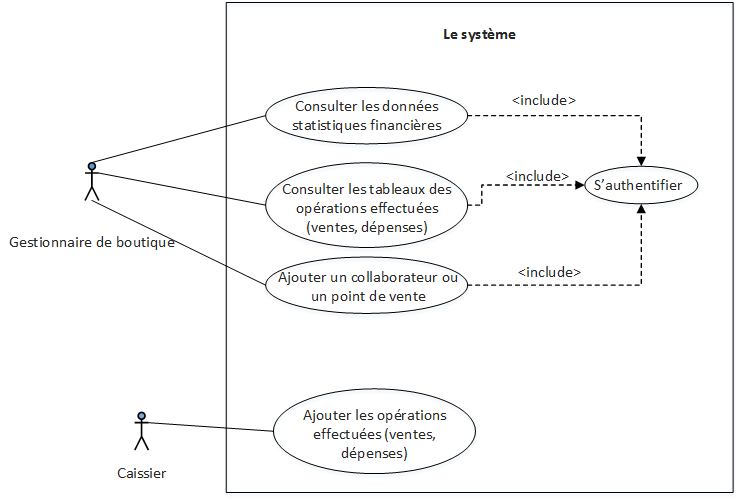
\includegraphics[scale=0.4, width=7cm, height=4.7cm]{images/diagramUserCase.png}
	\caption{Diagramme des cas d'utilisation}
	\end{figure} 
      \end{center}		  		
  \end{itemize}
  %============================================================================
  \end{frame}
  % END FRAME 7
    
    
  % DEBUT FRAME 8
  \begin{frame}
  %============================================================================
  \begin{itemize}
    \item Diagramme des classes
    
    \begin{center}
      \begin{figure}[H]
	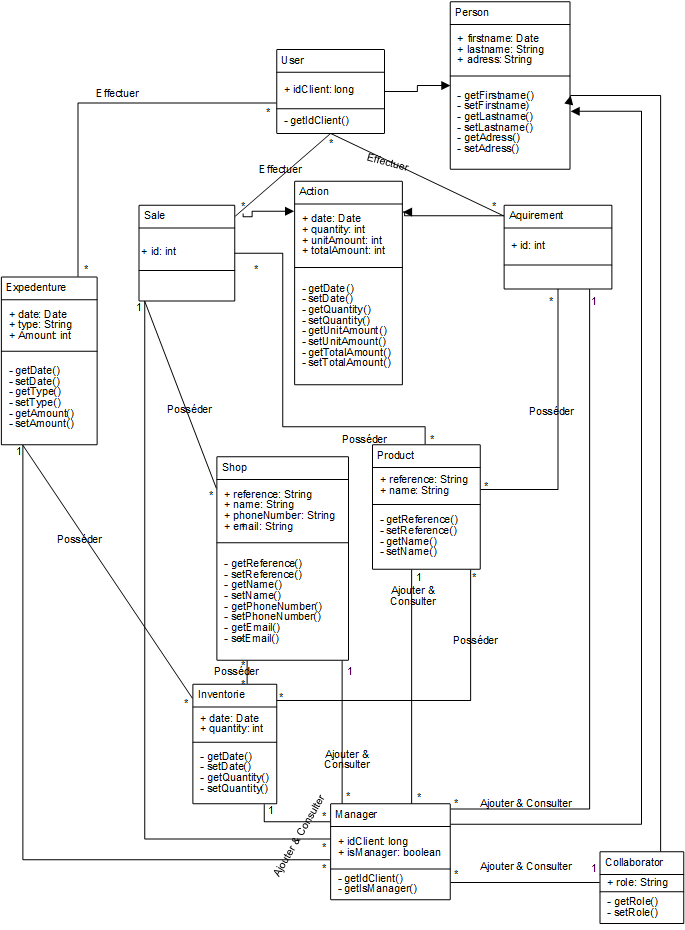
\includegraphics[scale=0.2, width=5cm]{images/diagramClass.png}
	\caption{Diagramme des classes}
      \end{figure} 
    \end{center}
  \end{itemize}
  %============================================================================
  \end{frame}
  % FIN FRAME 8
  
  % DEBUT FRAME 8
  \begin{frame}
  %============================================================================
  \begin{itemize}
    \item Diagramme de l'architecture
    
    \begin{center}
      \begin{figure}[H]
	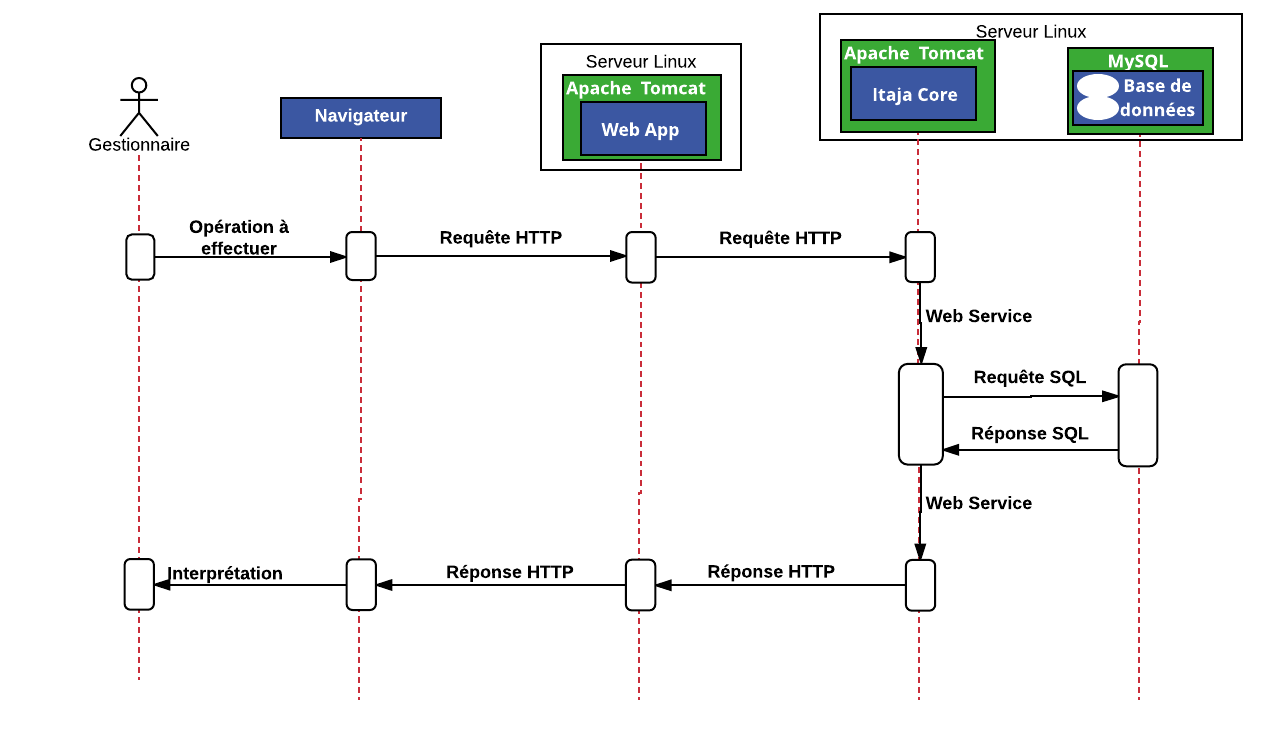
\includegraphics[scale=0.3, width=9cm]{images/diagramArchitecture.png}
	\caption{Diagramme de l'architecture}
      \end{figure} 
    \end{center}
  \end{itemize}
  %============================================================================
  \end{frame}
  % FIN FRAME 8
  
  % DEBUT FRAME 8
  \begin{frame}
  %============================================================================
  \begin{itemize}
    \item Diagramme de déployement
    
    \begin{center}
      \begin{figure}[H]
	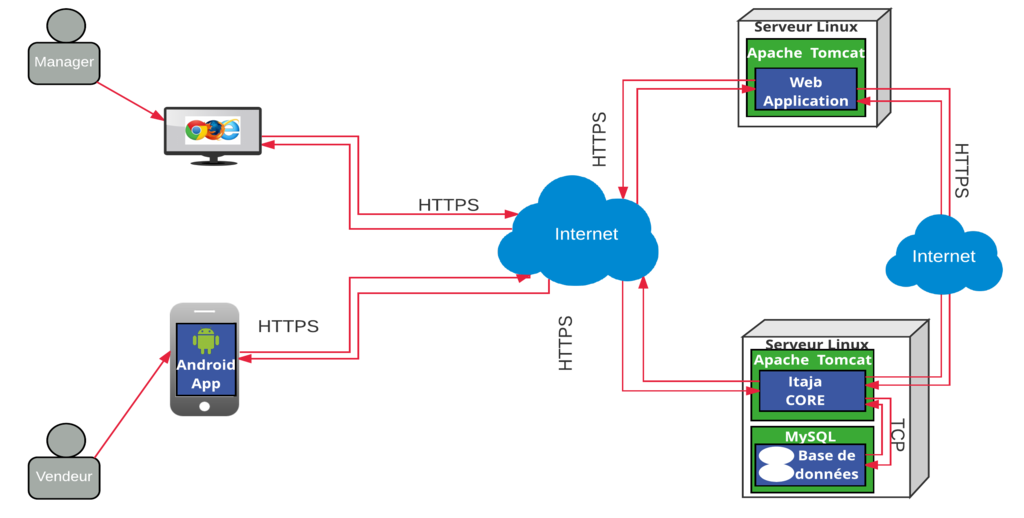
\includegraphics[scale=0.3, width=9cm]{images/diagrammeDeployement.png}
	\caption{Diagramme de déployement}
      \end{figure} 
    \end{center}
  \end{itemize}
  %============================================================================
  \end{frame}
  % FIN FRAME 8

  \subsection{Technologies utilisés}
  %\setbeamertemplate{frametitlecontinuation} {\insertcontinuationcount}
  % DEBUT FRAME 9
  \begin{frame}{Technologies utilisés}
  %============================================================================
  \begin{center}
    \begin{figure}[H]
      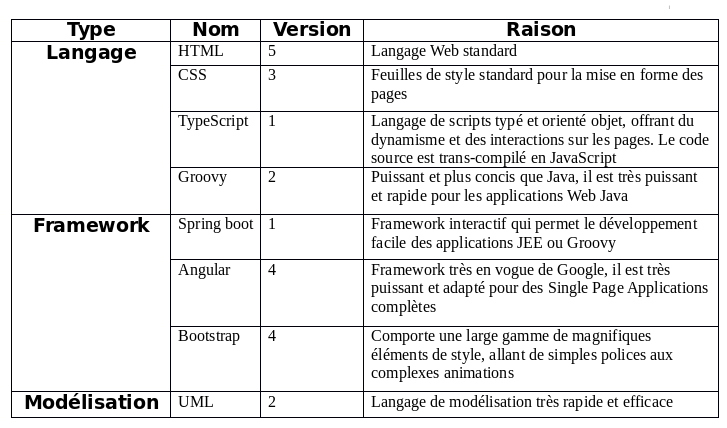
\includegraphics[scale=0.1, width=7cm, height=6cm]{images/resumeChoix.png}
      \caption{Résumé des choix technologiques}
    \end{figure} 
  \end{center}	
  %=============================================================================
  \end{frame}
  % FIN FRAME 12

  \subsection{Autres outils}
  %\setbeamertemplate{frametitlecontinuation} {\insertcontinuationcount}
  % DEBUT FRAME 9
  \begin{frame}{Autres outils}
  %============================================================================
  \begin{center}
    \begin{figure}[H]
      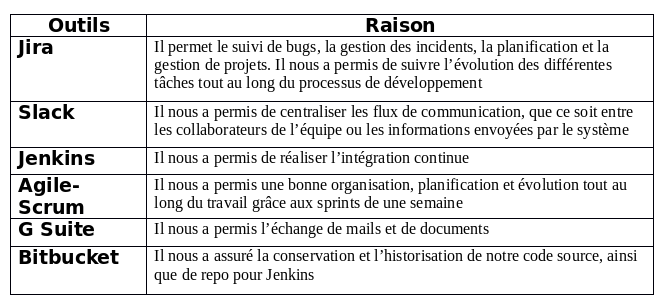
\includegraphics[scale=0.1, width=7cm, height=6cm]{images/resumeOutils.png}
      \caption{Résumé des outils de projets utilisés}
    \end{figure} 
  \end{center}	
  %=============================================================================
  \end{frame}
  % FIN FRAME 12
    
  \section{Résultats et Perspectives}
  \subsection{Résultats}
  % DEBUT FRAME 13
  \begin{frame}{Résultats}
  %=============================================================================
  \begin{center}
  \begin{figure}[H]
  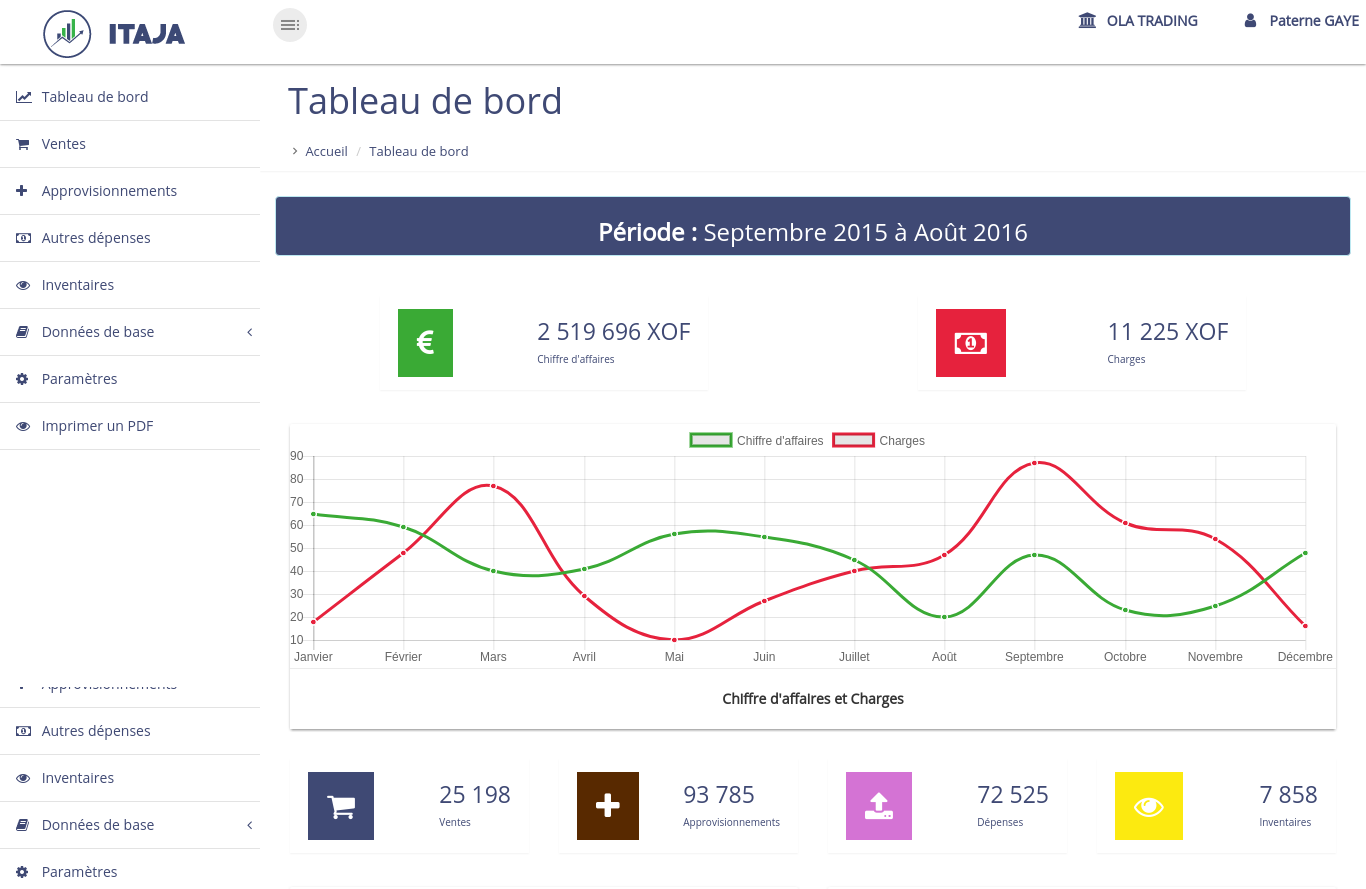
\includegraphics[scale=0.5, width=9cm]{images/qdashboard1.png}
  \caption{Présentation des statistiques financières(chiffre d'affaires, charges)}
  \end{figure} 
  \end{center}	
  \end{frame}
  
  \begin{frame}
  %=============================================================================
  \begin{center}
  \begin{figure}[H]
  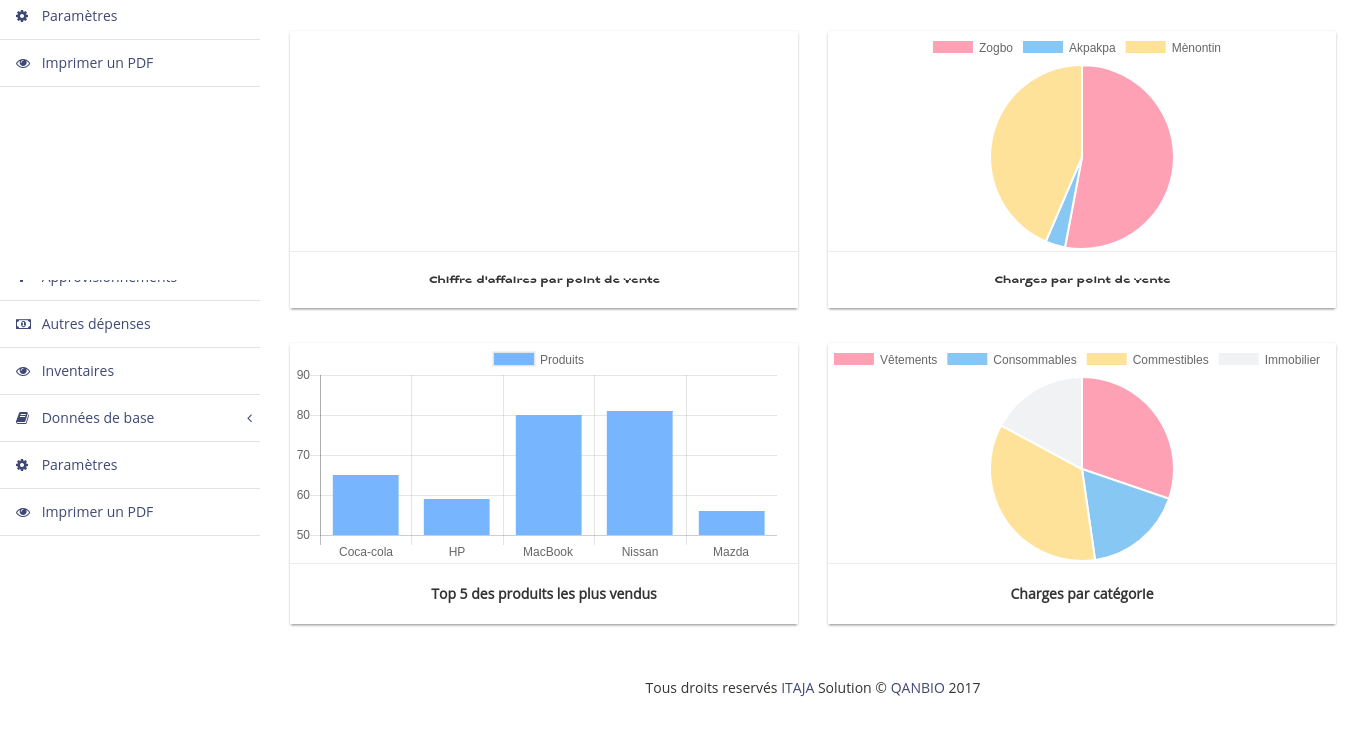
\includegraphics[scale=0.5, width=9cm]{images/qdashboard2.png}
  \caption{Présentation des indicateurs d'actions}
  \end{figure} 
  \end{center}	
  \end{frame}
  
  \begin{frame}
  %=============================================================================
  \begin{center}
  \begin{figure}[H]
  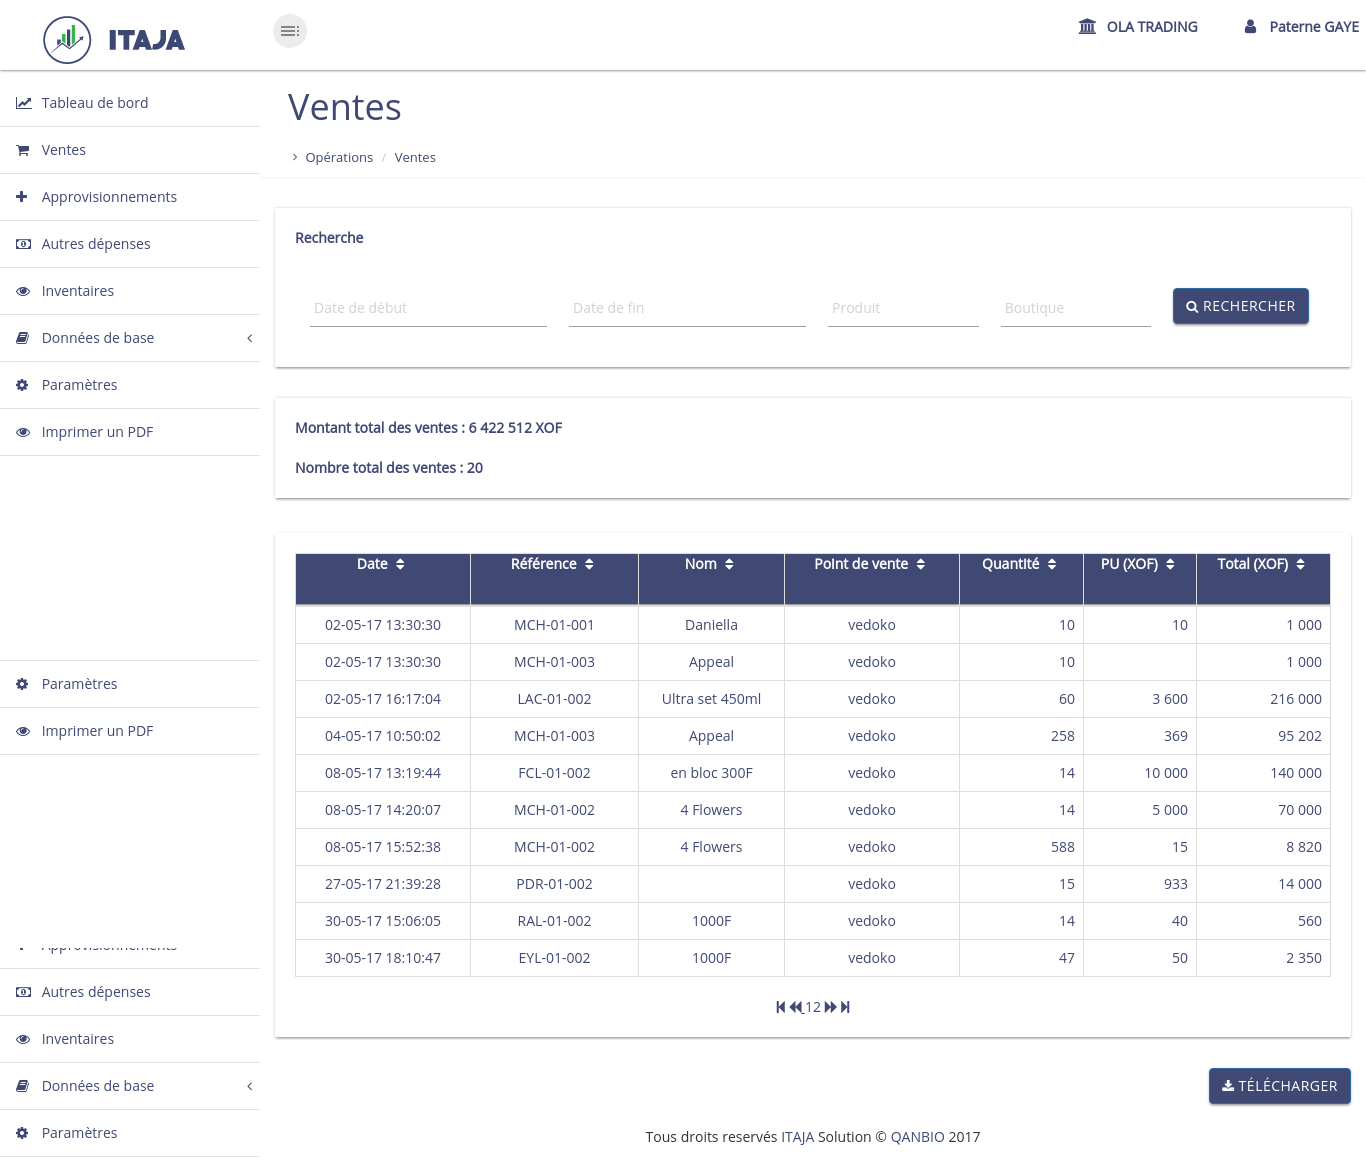
\includegraphics[scale=0.3, width=8cm]{images/qsales.png}
  \caption{Presentation du tableau des ventes}
  \end{figure} 
  \end{center}	
  \end{frame}
  
  \begin{frame}
  %=============================================================================
  \begin{center}
  \begin{figure}[H]
  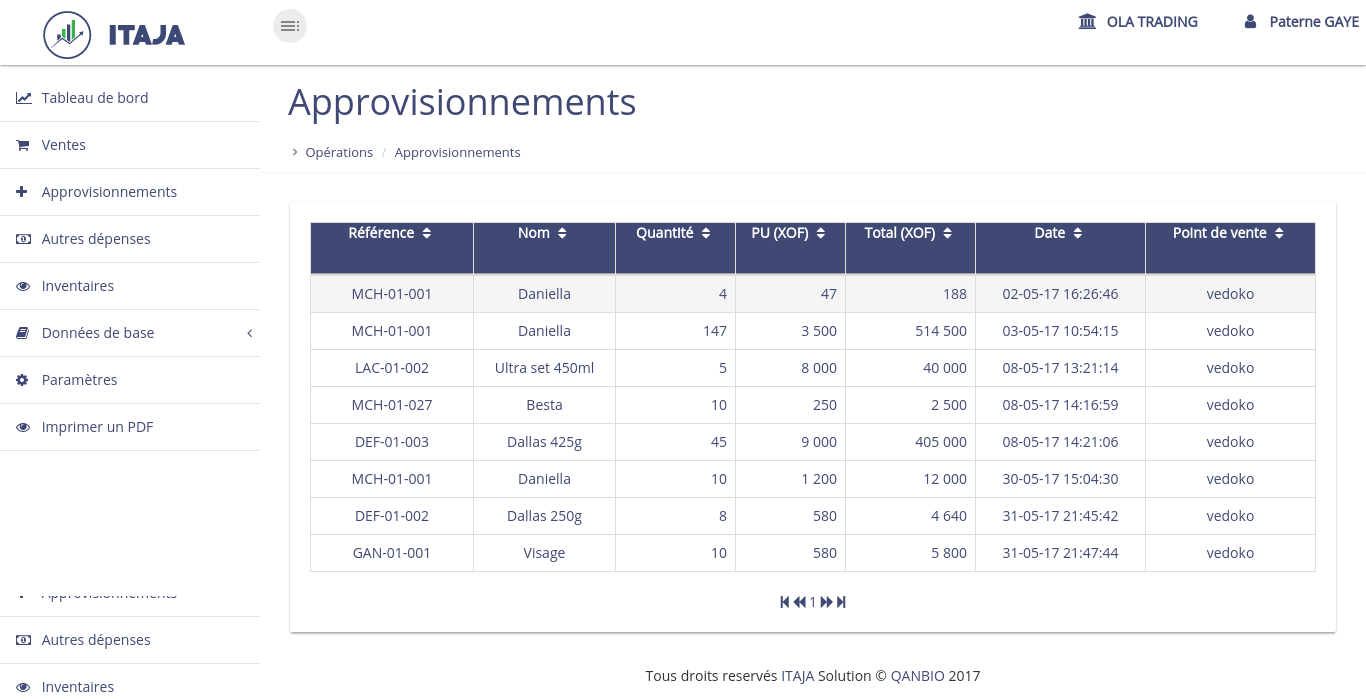
\includegraphics[scale=0.3, width=12cm]{images/qprocurements.png}
  \caption{Presentation du tableau des approvisionnements}
  \end{figure} 
  \end{center}	
  \end{frame}
  
  \subsection{Perspectives}
  %==============================================================================
  \begin{frame}{Perspectives}
  \begin{itemize}
  \item Ajout et suppression des collaborateurs et des points de ventes ;
  \pause
  \item Indexation automatique des produits et/ou zones qui méritent un investissement ou dont il faut arrêter l'exploitation ;
  \pause
  \item Prévision automatique du chiffre d'affaires sur une période donnée en fonction de l'évolution des ventes ;
  \end{itemize}
  %===============================================================================
  \end{frame}
  % DEBUT FRAME 13
    
  \section{Conclusion }
  % DEBUT FRAME 14
  \begin{frame}{Conclusion}
  %===============================================================================
  \begin{enumerate}
  \item Une expérience enrichissante (Angular, Spring Boot, Maven, Groovy, Jenkins...);
  \pause
  \item Le plaisir de proposer une application pour solutionner les problèmes de gestion de stocks et d'analyse financière des Très Petite Entreprise et des Petite et Moyenne Entreprise ;
  \pause
  \item La possibilité de savoir la zone ou le produit le plus ou le moins vendu ;
  \pause
  \item La possibilité d'avoir les statistiques d'une ou des boutiques sur une période donnée.
  \end{enumerate}
  %=============================================================================
  \end{frame}
  % FIN FRAME 14


  % DEBUT FRAME 15
  \begin{frame}{FIN}
  %=============================================================================
  \begin{center}
    Merci de votre aimable attention!
  \end{center}
  %=============================================================================
  \end{frame}   
  % FIN FRAME 15

  % FIN DU DOCUMENT
\end{document}